\documentclass[twoside]{book}

% Packages required by doxygen
\usepackage{fixltx2e}
\usepackage{calc}
\usepackage{doxygen}
\usepackage[export]{adjustbox} % also loads graphicx
\usepackage{graphicx}
\usepackage[utf8]{inputenc}
\usepackage{makeidx}
\usepackage{multicol}
\usepackage{multirow}
\PassOptionsToPackage{warn}{textcomp}
\usepackage{textcomp}
\usepackage[nointegrals]{wasysym}
\usepackage[table]{xcolor}

% Font selection
\usepackage[T1]{fontenc}
\usepackage[scaled=.90]{helvet}
\usepackage{courier}
\usepackage{amssymb}
\usepackage{sectsty}
\renewcommand{\familydefault}{\sfdefault}
\allsectionsfont{%
  \fontseries{bc}\selectfont%
  \color{darkgray}%
}
\renewcommand{\DoxyLabelFont}{%
  \fontseries{bc}\selectfont%
  \color{darkgray}%
}
\newcommand{\+}{\discretionary{\mbox{\scriptsize$\hookleftarrow$}}{}{}}

% Page & text layout
\usepackage{geometry}
\geometry{%
  a4paper,%
  top=2.5cm,%
  bottom=2.5cm,%
  left=2.5cm,%
  right=2.5cm%
}
\tolerance=750
\hfuzz=15pt
\hbadness=750
\setlength{\emergencystretch}{15pt}
\setlength{\parindent}{0cm}
\setlength{\parskip}{3ex plus 2ex minus 2ex}
\makeatletter
\renewcommand{\paragraph}{%
  \@startsection{paragraph}{4}{0ex}{-1.0ex}{1.0ex}{%
    \normalfont\normalsize\bfseries\SS@parafont%
  }%
}
\renewcommand{\subparagraph}{%
  \@startsection{subparagraph}{5}{0ex}{-1.0ex}{1.0ex}{%
    \normalfont\normalsize\bfseries\SS@subparafont%
  }%
}
\makeatother

% Headers & footers
\usepackage{fancyhdr}
\pagestyle{fancyplain}
\fancyhead[LE]{\fancyplain{}{\bfseries\thepage}}
\fancyhead[CE]{\fancyplain{}{}}
\fancyhead[RE]{\fancyplain{}{\bfseries\leftmark}}
\fancyhead[LO]{\fancyplain{}{\bfseries\rightmark}}
\fancyhead[CO]{\fancyplain{}{}}
\fancyhead[RO]{\fancyplain{}{\bfseries\thepage}}
\fancyfoot[LE]{\fancyplain{}{}}
\fancyfoot[CE]{\fancyplain{}{}}
\fancyfoot[RE]{\fancyplain{}{\bfseries\scriptsize Generated by Doxygen }}
\fancyfoot[LO]{\fancyplain{}{\bfseries\scriptsize Generated by Doxygen }}
\fancyfoot[CO]{\fancyplain{}{}}
\fancyfoot[RO]{\fancyplain{}{}}
\renewcommand{\footrulewidth}{0.4pt}
\renewcommand{\chaptermark}[1]{%
  \markboth{#1}{}%
}
\renewcommand{\sectionmark}[1]{%
  \markright{\thesection\ #1}%
}

% Indices & bibliography
\usepackage{natbib}
\usepackage[titles]{tocloft}
\setcounter{tocdepth}{3}
\setcounter{secnumdepth}{5}
\makeindex

% Hyperlinks (required, but should be loaded last)
\usepackage{ifpdf}
\ifpdf
  \usepackage[pdftex,pagebackref=true]{hyperref}
\else
  \usepackage[ps2pdf,pagebackref=true]{hyperref}
\fi
\hypersetup{%
  colorlinks=true,%
  linkcolor=blue,%
  citecolor=blue,%
  unicode%
}

% Custom commands
\newcommand{\clearemptydoublepage}{%
  \newpage{\pagestyle{empty}\cleardoublepage}%
}

\usepackage{caption}
\captionsetup{labelsep=space,justification=centering,font={bf},singlelinecheck=off,skip=4pt,position=top}

%===== C O N T E N T S =====

\begin{document}

% Titlepage & ToC
\hypersetup{pageanchor=false,
             bookmarksnumbered=true,
             pdfencoding=unicode
            }
\pagenumbering{roman}
\begin{titlepage}
\vspace*{7cm}
\begin{center}%
{\Large My Project }\\
\vspace*{1cm}
{\large Generated by Doxygen 1.8.11}\\
\end{center}
\end{titlepage}
\clearemptydoublepage
\tableofcontents
\clearemptydoublepage
\pagenumbering{arabic}
\hypersetup{pageanchor=true}

%--- Begin generated contents ---
\chapter{Hierarchical Index}
\section{Class Hierarchy}
This inheritance list is sorted roughly, but not completely, alphabetically\+:\begin{DoxyCompactList}
\item \contentsline{section}{Animal}{\pageref{classAnimal}}{}
\begin{DoxyCompactList}
\item \contentsline{section}{Dog}{\pageref{classDog}}{}
\item \contentsline{section}{Snake}{\pageref{classSnake}}{}
\begin{DoxyCompactList}
\item \contentsline{section}{Dangerous\+Snake}{\pageref{classDangerousSnake}}{}
\item \contentsline{section}{Non\+Dangerous\+Snake}{\pageref{classNonDangerousSnake}}{}
\begin{DoxyCompactList}
\item \contentsline{section}{Python}{\pageref{structPython}}{}
\end{DoxyCompactList}
\end{DoxyCompactList}
\end{DoxyCompactList}
\end{DoxyCompactList}

\chapter{Class Index}
\section{Class List}
Here are the classes, structs, unions and interfaces with brief descriptions\+:\begin{DoxyCompactList}
\item\contentsline{section}{\hyperlink{classAnimal}{Animal} }{\pageref{classAnimal}}{}
\item\contentsline{section}{\hyperlink{classDangerousSnake}{Dangerous\+Snake} }{\pageref{classDangerousSnake}}{}
\item\contentsline{section}{\hyperlink{classDog}{Dog} }{\pageref{classDog}}{}
\item\contentsline{section}{\hyperlink{classNonDangerousSnake}{Non\+Dangerous\+Snake} }{\pageref{classNonDangerousSnake}}{}
\item\contentsline{section}{\hyperlink{structPython}{Python} }{\pageref{structPython}}{}
\item\contentsline{section}{\hyperlink{classSnake}{Snake} }{\pageref{classSnake}}{}
\end{DoxyCompactList}

\chapter{Class Documentation}
\hypertarget{classAnimal}{}\section{Animal Class Reference}
\label{classAnimal}\index{Animal@{Animal}}


{\ttfamily \#include $<$animal.\+h$>$}

Inheritance diagram for Animal\+:\begin{figure}[H]
\begin{center}
\leavevmode
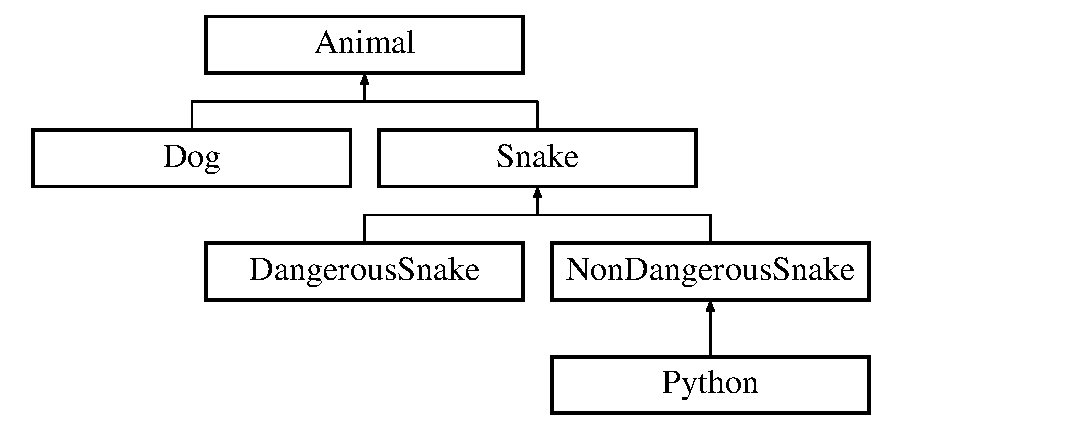
\includegraphics[height=4.000000cm]{classAnimal}
\end{center}
\end{figure}
\subsection*{Public Member Functions}
\begin{DoxyCompactItemize}
\item 
\hyperlink{classAnimal_aaf54366e9bfa8730f100fd25b99b864f}{Animal} (const unsigned int a, const double w)
\item 
\hyperlink{classAnimal_a1e726a49ec952443190ac62dad22353c}{Animal} ()
\item 
virtual void \hyperlink{classAnimal_ae3f640ffd5ebec66c3836b63fd11fc27}{speak} () const =0
\item 
virtual void \hyperlink{classAnimal_a72994a2bb769667d277845351462246f}{info} () const noexcept
\item 
virtual \hyperlink{classAnimal_a16d8b7f94611cc65f5cdb58cc105527b}{$\sim$\+Animal} ()
\end{DoxyCompactItemize}


\subsection{Detailed Description}
Base class for animals. Each new animal should derive from this class and override {\ttfamily \hyperlink{classAnimal_ae3f640ffd5ebec66c3836b63fd11fc27}{speak()}} which is pure virtual. 

\subsection{Constructor \& Destructor Documentation}
\index{Animal@{Animal}!Animal@{Animal}}
\index{Animal@{Animal}!Animal@{Animal}}
\subsubsection[{\texorpdfstring{Animal(const unsigned int a, const double w)}{Animal(const unsigned int a, const double w)}}]{\setlength{\rightskip}{0pt plus 5cm}Animal\+::\+Animal (
\begin{DoxyParamCaption}
\item[{const unsigned int}]{a, }
\item[{const double}]{w}
\end{DoxyParamCaption}
)}\hypertarget{classAnimal_aaf54366e9bfa8730f100fd25b99b864f}{}\label{classAnimal_aaf54366e9bfa8730f100fd25b99b864f}
\hyperlink{classAnimal}{Animal} Constructor. Takes {\ttfamily a} for the age and {\ttfamily w} for the weight. \index{Animal@{Animal}!Animal@{Animal}}
\index{Animal@{Animal}!Animal@{Animal}}
\subsubsection[{\texorpdfstring{Animal()}{Animal()}}]{\setlength{\rightskip}{0pt plus 5cm}Animal\+::\+Animal (
\begin{DoxyParamCaption}
{}
\end{DoxyParamCaption}
)}\hypertarget{classAnimal_a1e726a49ec952443190ac62dad22353c}{}\label{classAnimal_a1e726a49ec952443190ac62dad22353c}
Deafult constructor. Set all attributes to zero. \index{Animal@{Animal}!````~Animal@{$\sim$\+Animal}}
\index{````~Animal@{$\sim$\+Animal}!Animal@{Animal}}
\subsubsection[{\texorpdfstring{$\sim$\+Animal()}{~Animal()}}]{\setlength{\rightskip}{0pt plus 5cm}virtual Animal\+::$\sim$\+Animal (
\begin{DoxyParamCaption}
{}
\end{DoxyParamCaption}
)\hspace{0.3cm}{\ttfamily [inline]}, {\ttfamily [virtual]}}\hypertarget{classAnimal_a16d8b7f94611cc65f5cdb58cc105527b}{}\label{classAnimal_a16d8b7f94611cc65f5cdb58cc105527b}
Destructor. It does anything but is set virtual to ensure proper cleanup of the data that will be defined in the derived classes. 

\subsection{Member Function Documentation}
\index{Animal@{Animal}!info@{info}}
\index{info@{info}!Animal@{Animal}}
\subsubsection[{\texorpdfstring{info() const noexcept}{info() const noexcept}}]{\setlength{\rightskip}{0pt plus 5cm}void Animal\+::info (
\begin{DoxyParamCaption}
{}
\end{DoxyParamCaption}
) const\hspace{0.3cm}{\ttfamily [virtual]}, {\ttfamily [noexcept]}}\hypertarget{classAnimal_a72994a2bb769667d277845351462246f}{}\label{classAnimal_a72994a2bb769667d277845351462246f}
print animal\textquotesingle{}s details 

Reimplemented in \hyperlink{classSnake_a274887b6614bede92d3343c740f24206}{Snake}.

\index{Animal@{Animal}!speak@{speak}}
\index{speak@{speak}!Animal@{Animal}}
\subsubsection[{\texorpdfstring{speak() const =0}{speak() const =0}}]{\setlength{\rightskip}{0pt plus 5cm}virtual void Animal\+::speak (
\begin{DoxyParamCaption}
{}
\end{DoxyParamCaption}
) const\hspace{0.3cm}{\ttfamily [pure virtual]}}\hypertarget{classAnimal_ae3f640ffd5ebec66c3836b63fd11fc27}{}\label{classAnimal_ae3f640ffd5ebec66c3836b63fd11fc27}
print on stdout the animal\textquotesingle{}s call 

Implemented in \hyperlink{classSnake_a70ce47696989febece8de5280fa28aa7}{Snake}, and \hyperlink{classDog_a51416c2bf93f9f0f9be5b31d0c4d0dc8}{Dog}.



The documentation for this class was generated from the following files\+:\begin{DoxyCompactItemize}
\item 
/home/ginevracoal/\+M\+E\+G\+A/\+Università/\+D\+S\+S\+C/semester\+\_\+1/advanced\+\_\+programming/advanced-\/programming/lectures/06\+\_\+inheritance/organized/include/animal.\+h\item 
/home/ginevracoal/\+M\+E\+G\+A/\+Università/\+D\+S\+S\+C/semester\+\_\+1/advanced\+\_\+programming/advanced-\/programming/lectures/06\+\_\+inheritance/organized/src/animal.\+cc\end{DoxyCompactItemize}

\hypertarget{classDangerousSnake}{}\section{Dangerous\+Snake Class Reference}
\label{classDangerousSnake}\index{Dangerous\+Snake@{Dangerous\+Snake}}


{\ttfamily \#include $<$snake.\+h$>$}

Inheritance diagram for Dangerous\+Snake\+:\begin{figure}[H]
\begin{center}
\leavevmode
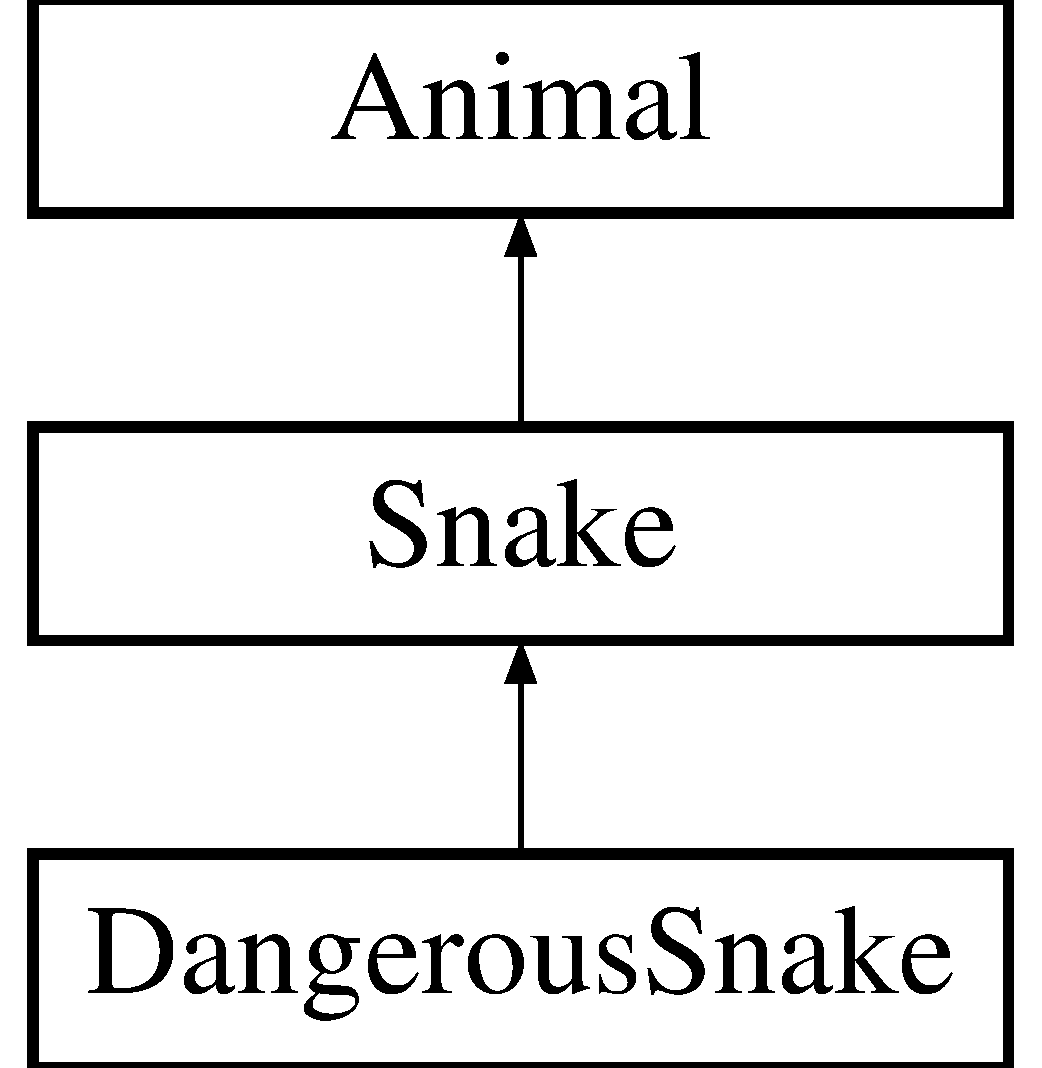
\includegraphics[height=3.000000cm]{classDangerousSnake}
\end{center}
\end{figure}
\subsection*{Public Member Functions}
\begin{DoxyCompactItemize}
\item 
{\bfseries Dangerous\+Snake} (const unsigned int a, const double w)\hypertarget{classDangerousSnake_affea07d2d8e6bcb61ee192cca2a05838}{}\label{classDangerousSnake_affea07d2d8e6bcb61ee192cca2a05838}

\end{DoxyCompactItemize}


\subsection{Detailed Description}
Specialization of class \hyperlink{classSnake}{Snake}. It specialize the constructors such that the attribute {\ttfamily dangerous} is set to true 

The documentation for this class was generated from the following file\+:\begin{DoxyCompactItemize}
\item 
/home/ginevracoal/\+M\+E\+G\+A/\+Università/\+D\+S\+S\+C/semester\+\_\+1/advanced\+\_\+programming/advanced-\/programming/lectures/06\+\_\+inheritance/organized/include/snake.\+h\end{DoxyCompactItemize}

\hypertarget{classDog}{}\section{Dog Class Reference}
\label{classDog}\index{Dog@{Dog}}


{\ttfamily \#include $<$dog.\+h$>$}

Inheritance diagram for Dog\+:\begin{figure}[H]
\begin{center}
\leavevmode
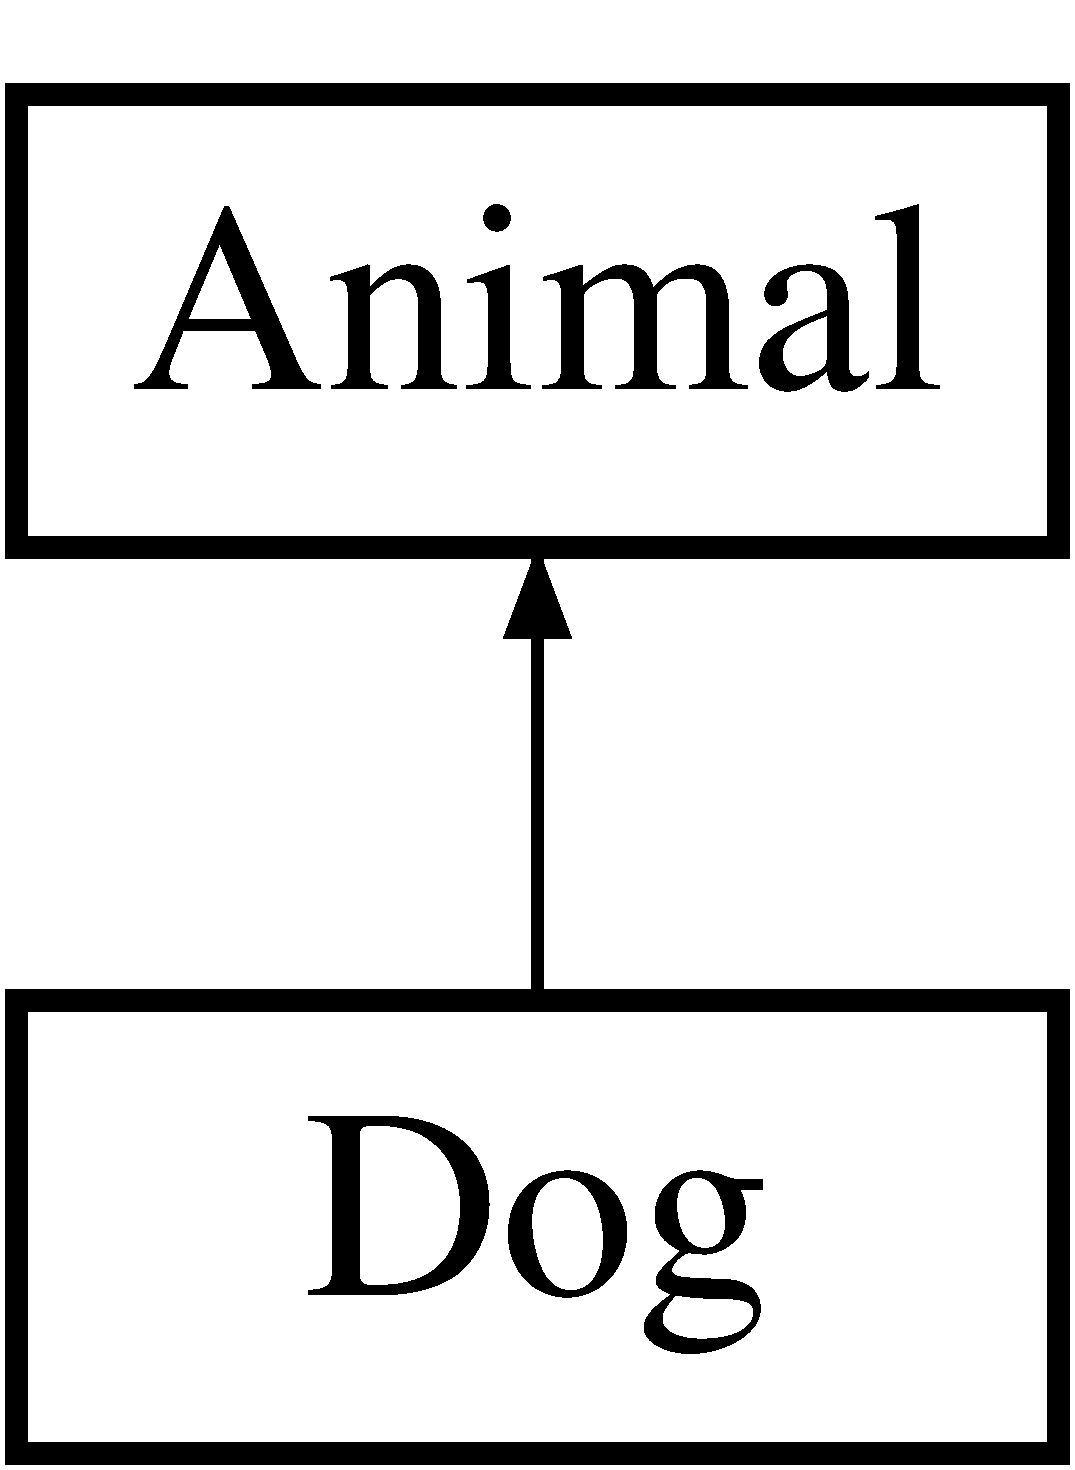
\includegraphics[height=2.000000cm]{classDog}
\end{center}
\end{figure}
\subsection*{Public Member Functions}
\begin{DoxyCompactItemize}
\item 
void \hyperlink{classDog_a51416c2bf93f9f0f9be5b31d0c4d0dc8}{speak} () const noexceptoverride
\item 
\hyperlink{classDog_a36b671ae98da1a176dd3fd295874c3ec}{Dog} ()=default
\item 
\hyperlink{classDog_a1b72afe034eb61f5de9af43a9c8dad6f}{Dog} (const unsigned int a, const double d)
\end{DoxyCompactItemize}


\subsection{Detailed Description}
Specialization of class \hyperlink{classAnimal}{Animal}. It simply overrides the function speak. 

\subsection{Constructor \& Destructor Documentation}
\index{Dog@{Dog}!Dog@{Dog}}
\index{Dog@{Dog}!Dog@{Dog}}
\subsubsection[{\texorpdfstring{Dog()=default}{Dog()=default}}]{\setlength{\rightskip}{0pt plus 5cm}Dog\+::\+Dog (
\begin{DoxyParamCaption}
{}
\end{DoxyParamCaption}
)\hspace{0.3cm}{\ttfamily [default]}}\hypertarget{classDog_a36b671ae98da1a176dd3fd295874c3ec}{}\label{classDog_a36b671ae98da1a176dd3fd295874c3ec}
Default constructor is fine. It will call the default constructor of \hyperlink{classAnimal}{Animal}. \index{Dog@{Dog}!Dog@{Dog}}
\index{Dog@{Dog}!Dog@{Dog}}
\subsubsection[{\texorpdfstring{Dog(const unsigned int a, const double d)}{Dog(const unsigned int a, const double d)}}]{\setlength{\rightskip}{0pt plus 5cm}Dog\+::\+Dog (
\begin{DoxyParamCaption}
\item[{const unsigned int}]{a, }
\item[{const double}]{d}
\end{DoxyParamCaption}
)}\hypertarget{classDog_a1b72afe034eb61f5de9af43a9c8dad6f}{}\label{classDog_a1b72afe034eb61f5de9af43a9c8dad6f}
Delegating constructor to build an \hyperlink{classAnimal}{Animal}\{a,b\} 

\subsection{Member Function Documentation}
\index{Dog@{Dog}!speak@{speak}}
\index{speak@{speak}!Dog@{Dog}}
\subsubsection[{\texorpdfstring{speak() const noexceptoverride}{speak() const noexceptoverride}}]{\setlength{\rightskip}{0pt plus 5cm}void Dog\+::speak (
\begin{DoxyParamCaption}
{}
\end{DoxyParamCaption}
) const\hspace{0.3cm}{\ttfamily [override]}, {\ttfamily [virtual]}, {\ttfamily [noexcept]}}\hypertarget{classDog_a51416c2bf93f9f0f9be5b31d0c4d0dc8}{}\label{classDog_a51416c2bf93f9f0f9be5b31d0c4d0dc8}
A dog usually says \char`\"{}\+Bau\char`\"{} 

Implements \hyperlink{classAnimal_ae3f640ffd5ebec66c3836b63fd11fc27}{Animal}.



The documentation for this class was generated from the following files\+:\begin{DoxyCompactItemize}
\item 
/home/ginevracoal/\+M\+E\+G\+A/\+Università/\+D\+S\+S\+C/semester\+\_\+1/advanced\+\_\+programming/advanced-\/programming/lectures/06\+\_\+inheritance/organized/include/dog.\+h\item 
/home/ginevracoal/\+M\+E\+G\+A/\+Università/\+D\+S\+S\+C/semester\+\_\+1/advanced\+\_\+programming/advanced-\/programming/lectures/06\+\_\+inheritance/organized/src/dog.\+cc\end{DoxyCompactItemize}

\hypertarget{classNonDangerousSnake}{}\section{Non\+Dangerous\+Snake Class Reference}
\label{classNonDangerousSnake}\index{Non\+Dangerous\+Snake@{Non\+Dangerous\+Snake}}


{\ttfamily \#include $<$snake.\+h$>$}

Inheritance diagram for Non\+Dangerous\+Snake\+:\begin{figure}[H]
\begin{center}
\leavevmode
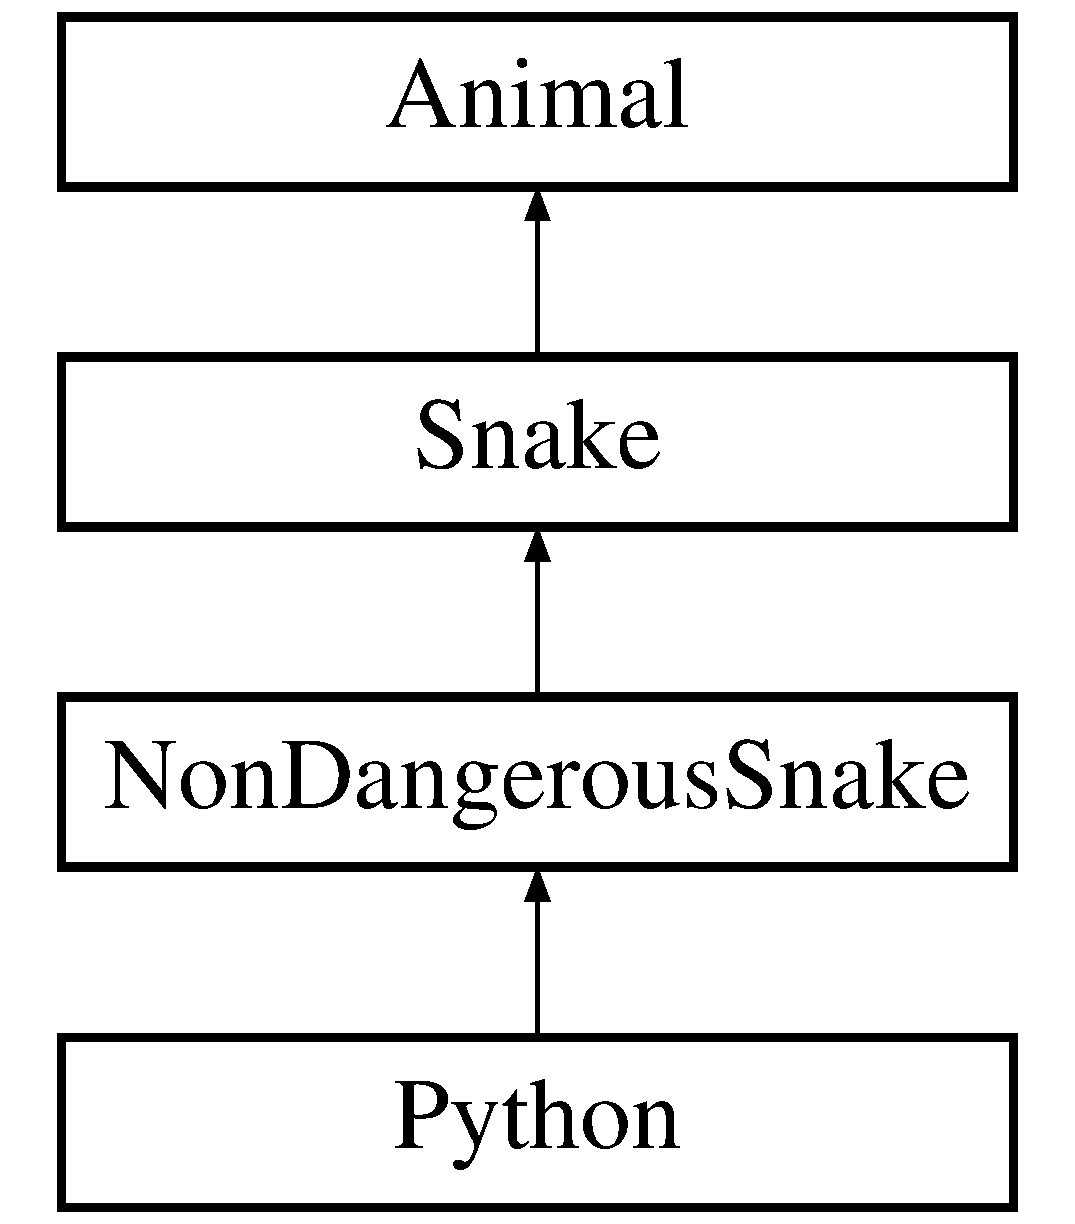
\includegraphics[height=4.000000cm]{classNonDangerousSnake}
\end{center}
\end{figure}
\subsection*{Public Member Functions}
\begin{DoxyCompactItemize}
\item 
{\bfseries Non\+Dangerous\+Snake} (const unsigned int a, const double w)\hypertarget{classNonDangerousSnake_a3f5ac2522dd02fc5d55a34f30eec7e43}{}\label{classNonDangerousSnake_a3f5ac2522dd02fc5d55a34f30eec7e43}

\end{DoxyCompactItemize}


\subsection{Detailed Description}
Specialization of class \hyperlink{classSnake}{Snake}. It specialize the constructors such that the attribute {\ttfamily dangerous} is set to false. 

The documentation for this class was generated from the following file\+:\begin{DoxyCompactItemize}
\item 
/home/ginevracoal/\+M\+E\+G\+A/\+Università/\+D\+S\+S\+C/semester\+\_\+1/advanced\+\_\+programming/advanced-\/programming/lectures/06\+\_\+inheritance/organized/include/snake.\+h\end{DoxyCompactItemize}

\hypertarget{structPython}{}\section{Python Struct Reference}
\label{structPython}\index{Python@{Python}}


{\ttfamily \#include $<$snake.\+h$>$}

Inheritance diagram for Python\+:\begin{figure}[H]
\begin{center}
\leavevmode
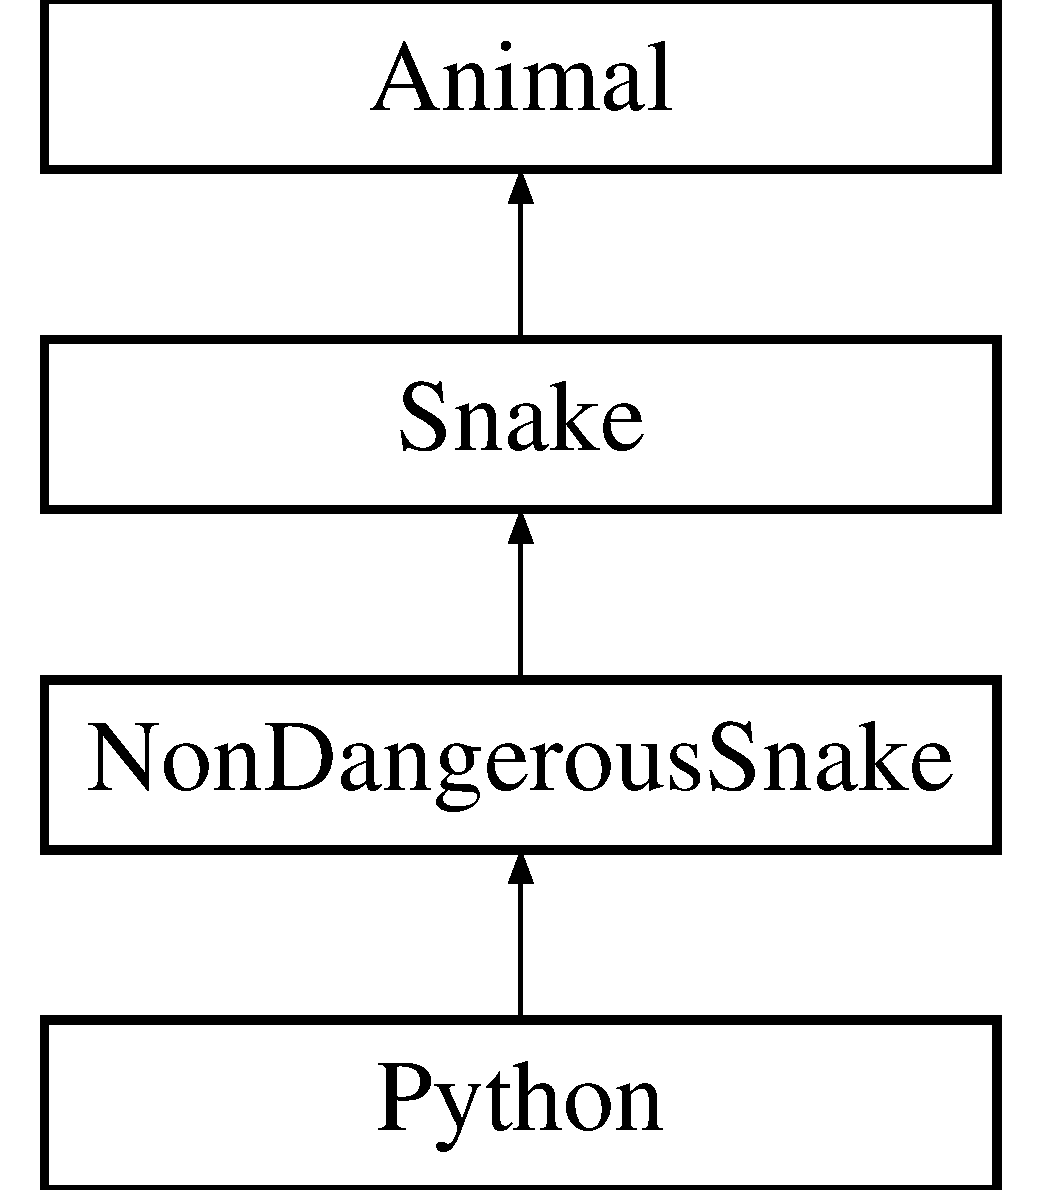
\includegraphics[height=4.000000cm]{structPython}
\end{center}
\end{figure}
\subsection*{Additional Inherited Members}


\subsection{Detailed Description}
Define the type \hyperlink{structPython}{Python} 

The documentation for this struct was generated from the following file\+:\begin{DoxyCompactItemize}
\item 
/home/ginevracoal/\+M\+E\+G\+A/\+Università/\+D\+S\+S\+C/semester\+\_\+1/advanced\+\_\+programming/advanced-\/programming/lectures/06\+\_\+inheritance/organized/include/snake.\+h\end{DoxyCompactItemize}

\hypertarget{classSnake}{}\section{Snake Class Reference}
\label{classSnake}\index{Snake@{Snake}}


{\ttfamily \#include $<$snake.\+h$>$}

Inheritance diagram for Snake\+:\begin{figure}[H]
\begin{center}
\leavevmode
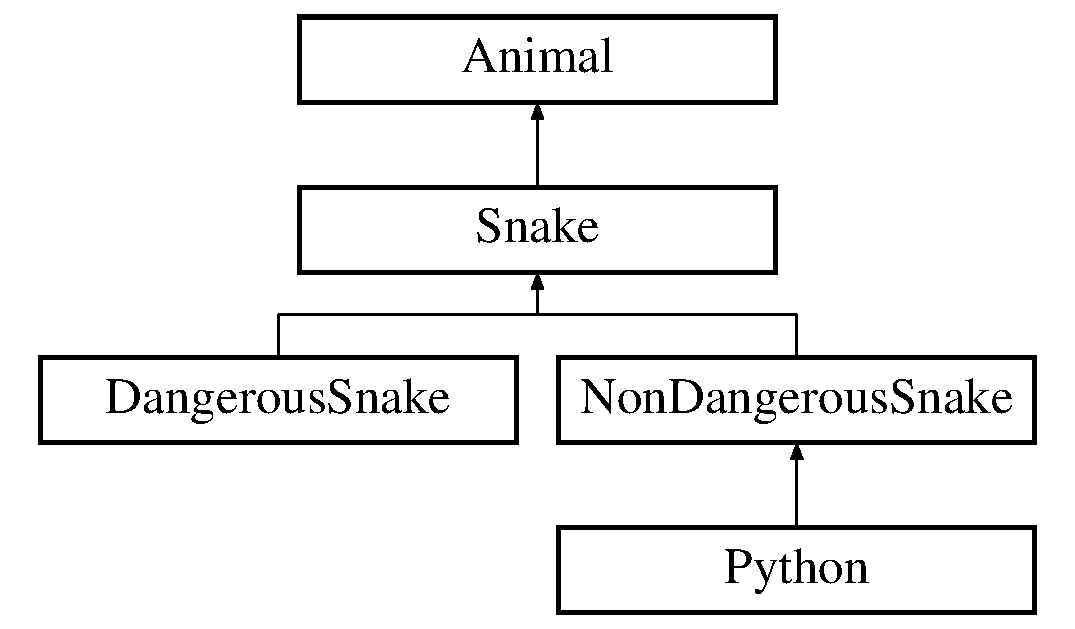
\includegraphics[height=4.000000cm]{classSnake}
\end{center}
\end{figure}
\subsection*{Public Member Functions}
\begin{DoxyCompactItemize}
\item 
\hyperlink{classSnake_a57f45c42d54f744517283ed5411f01d7}{Snake} (const unsigned int a, const double w, const bool b)
\item 
\hyperlink{classSnake_a3155ff2573c745c17c8b8ca8b90b5926}{Snake} (const bool b)
\item 
void \hyperlink{classSnake_a274887b6614bede92d3343c740f24206}{info} () const noexceptoverride
\item 
void \hyperlink{classSnake_a70ce47696989febece8de5280fa28aa7}{speak} () const noexceptoverride
\end{DoxyCompactItemize}


\subsection{Detailed Description}
Base class for snakes. It specializes into \hyperlink{classDangerousSnake}{Dangerous\+Snake} and \hyperlink{classNonDangerousSnake}{Non\+Dangerous\+Snake}. It is derived from class \hyperlink{classAnimal}{Animal} and add a boolean Snake\+::dangerous to specify if a type of snake is dangerous or not. 

\subsection{Constructor \& Destructor Documentation}
\index{Snake@{Snake}!Snake@{Snake}}
\index{Snake@{Snake}!Snake@{Snake}}
\subsubsection[{\texorpdfstring{Snake(const unsigned int a, const double w, const bool b)}{Snake(const unsigned int a, const double w, const bool b)}}]{\setlength{\rightskip}{0pt plus 5cm}Snake\+::\+Snake (
\begin{DoxyParamCaption}
\item[{const unsigned int}]{a, }
\item[{const double}]{w, }
\item[{const bool}]{b}
\end{DoxyParamCaption}
)}\hypertarget{classSnake_a57f45c42d54f744517283ed5411f01d7}{}\label{classSnake_a57f45c42d54f744517283ed5411f01d7}
Constructor. Takes all the arguments to construct an \hyperlink{classAnimal}{Animal} plus the additional boolean \index{Snake@{Snake}!Snake@{Snake}}
\index{Snake@{Snake}!Snake@{Snake}}
\subsubsection[{\texorpdfstring{Snake(const bool b)}{Snake(const bool b)}}]{\setlength{\rightskip}{0pt plus 5cm}Snake\+::\+Snake (
\begin{DoxyParamCaption}
\item[{const bool}]{b}
\end{DoxyParamCaption}
)}\hypertarget{classSnake_a3155ff2573c745c17c8b8ca8b90b5926}{}\label{classSnake_a3155ff2573c745c17c8b8ca8b90b5926}
Calls the default constructor for \hyperlink{classAnimal}{Animal}, and the {\ttfamily dangerous} is set to {\ttfamily b} 

\subsection{Member Function Documentation}
\index{Snake@{Snake}!info@{info}}
\index{info@{info}!Snake@{Snake}}
\subsubsection[{\texorpdfstring{info() const noexceptoverride}{info() const noexceptoverride}}]{\setlength{\rightskip}{0pt plus 5cm}void Snake\+::info (
\begin{DoxyParamCaption}
{}
\end{DoxyParamCaption}
) const\hspace{0.3cm}{\ttfamily [override]}, {\ttfamily [virtual]}, {\ttfamily [noexcept]}}\hypertarget{classSnake_a274887b6614bede92d3343c740f24206}{}\label{classSnake_a274887b6614bede92d3343c740f24206}
Print details. 

Reimplemented from \hyperlink{classAnimal_a72994a2bb769667d277845351462246f}{Animal}.

\index{Snake@{Snake}!speak@{speak}}
\index{speak@{speak}!Snake@{Snake}}
\subsubsection[{\texorpdfstring{speak() const noexceptoverride}{speak() const noexceptoverride}}]{\setlength{\rightskip}{0pt plus 5cm}void Snake\+::speak (
\begin{DoxyParamCaption}
{}
\end{DoxyParamCaption}
) const\hspace{0.3cm}{\ttfamily [override]}, {\ttfamily [virtual]}, {\ttfamily [noexcept]}}\hypertarget{classSnake_a70ce47696989febece8de5280fa28aa7}{}\label{classSnake_a70ce47696989febece8de5280fa28aa7}
\hyperlink{classSnake}{Snake}\textquotesingle{}s call 

Implements \hyperlink{classAnimal_ae3f640ffd5ebec66c3836b63fd11fc27}{Animal}.



The documentation for this class was generated from the following files\+:\begin{DoxyCompactItemize}
\item 
/home/ginevracoal/\+M\+E\+G\+A/\+Università/\+D\+S\+S\+C/semester\+\_\+1/advanced\+\_\+programming/advanced-\/programming/lectures/06\+\_\+inheritance/organized/include/snake.\+h\item 
/home/ginevracoal/\+M\+E\+G\+A/\+Università/\+D\+S\+S\+C/semester\+\_\+1/advanced\+\_\+programming/advanced-\/programming/lectures/06\+\_\+inheritance/organized/src/snake.\+cc\end{DoxyCompactItemize}

%--- End generated contents ---

% Index
\backmatter
\newpage
\phantomsection
\clearemptydoublepage
\addcontentsline{toc}{chapter}{Index}
\printindex

\end{document}
